\section{Experiments}
\label{sec:experiments}

We organize the experiments around five research questions. Unless otherwise stated, the current full-graph closure uses NetHEPT under the independent-cascade model with $|V|=15{,}233$, seed budget $k=10$, an independent 50k-RR screening sketch, shortlist size $M=128$, and 1,000 Monte Carlo worlds for final spread evaluation. Reported closure numbers use three independent repeats.

\begin{figure}[t]
    \centering
    \resizebox{0.98\linewidth}{!}{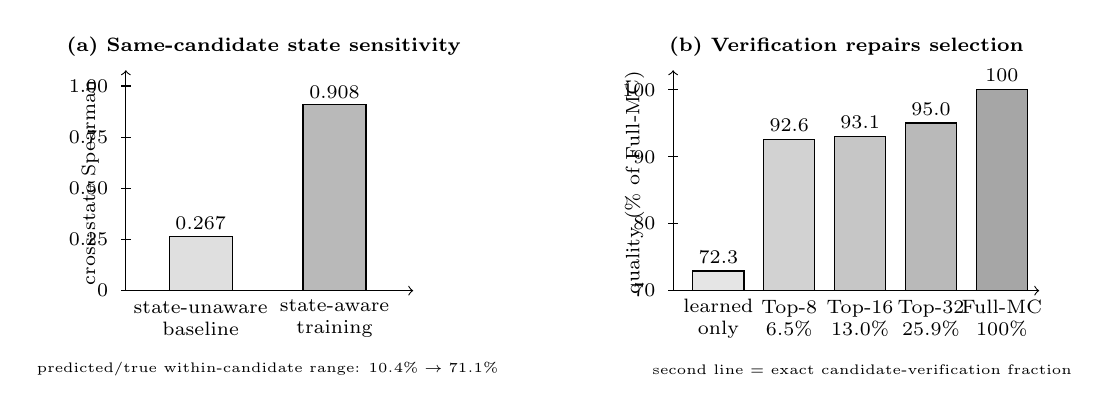
\begin{tikzpicture}[font=\scriptsize]
% Panel (a): state awareness
\begin{scope}[xshift=0cm]
  \node[font=\scriptsize\bfseries] at (2.15,3.55) {(a) Same-candidate state sensitivity};
  \draw[->] (0.4,0.45) -- (0.4,3.25);
  \draw[->] (0.4,0.45) -- (4.05,0.45);
  \foreach \y/\lab in {0.45/0,1.10/0.25,1.75/0.50,2.40/0.75,3.05/1.00}{
    \draw (0.34,\y)--(0.46,\y); \node[anchor=east] at (0.30,\y) {\lab};
  }
  \filldraw[fill=gray!25] (0.95,0.45) rectangle (1.75,1.14);
  \filldraw[fill=gray!55] (2.65,0.45) rectangle (3.45,2.81);
  \node at (1.35,1.30) {0.267};
  \node at (3.05,2.97) {0.908};
  \node[align=center] at (1.35,0.10) {state-unaware\\baseline};
  \node[align=center] at (3.05,0.10) {state-aware\\training};
  \node[rotate=90] at (-0.05,1.82) {cross-state Spearman};
  \node[align=center, font=\tiny] at (2.2,-0.55) {predicted/true within-candidate range: $10.4\%\rightarrow71.1\%$};
\end{scope}

% Panel (b): verification repairs sequential selection
\begin{scope}[xshift=7.0cm]
  \node[font=\scriptsize\bfseries] at (2.55,3.55) {(b) Verification repairs selection};
  \draw[->] (0.35,0.45) -- (0.35,3.25);
  \draw[->] (0.35,0.45) -- (5.0,0.45);
  \foreach \y/\lab in {0.45/70,1.30/80,2.15/90,3.00/100}{
    \draw (0.29,\y)--(0.41,\y); \node[anchor=east] at (0.25,\y) {\lab};
  }
  \def\base{0.45}
  % height mapping: y=0.45 + (quality-70)*0.085
  \filldraw[fill=gray!20] (0.60,0.45) rectangle (1.25,0.70);
  \filldraw[fill=gray!35] (1.50,0.45) rectangle (2.15,2.37);
  \filldraw[fill=gray!45] (2.40,0.45) rectangle (3.05,2.41);
  \filldraw[fill=gray!55] (3.30,0.45) rectangle (3.95,2.58);
  \filldraw[fill=gray!70] (4.20,0.45) rectangle (4.85,3.00);
  \node at (0.925,0.88) {72.3};
  \node at (1.825,2.55) {92.6};
  \node at (2.725,2.59) {93.1};
  \node at (3.625,2.76) {95.0};
  \node at (4.525,3.18) {100};
  \node[align=center] at (0.925,0.10) {learned\\only};
  \node[align=center] at (1.825,0.10) {Top-8\\$6.5\%$};
  \node[align=center] at (2.725,0.10) {Top-16\\$13.0\%$};
  \node[align=center] at (3.625,0.10) {Top-32\\$25.9\%$};
  \node[align=center] at (4.525,0.10) {Full-MC\\$100\%$};
  \node[rotate=90] at (-0.14,1.82) {quality (\% of Full-MC)};
  \node[font=\tiny] at (2.75,-0.55) {second line = exact candidate-verification fraction};
\end{scope}
\end{tikzpicture}
}
    \caption{Diagnostics motivating the design. \textbf{(a)} State-aware supervision raises same-candidate cross-state Spearman from $0.267$ to $0.908$ and restores the response to diminishing returns. \textbf{(b)} Learned-only sequential selection reaches only about $72\%$ of Full-MC quality; selectively verifying the predicted head recovers $92.6$--$95.0\%$ as verification increases.}
    \label{fig:diagnostics}
\end{figure}

\paragraph{RQ1: Is learned marginal gain genuinely state aware?}
Figure~\ref{fig:diagnostics}(a) evaluates the same candidate under multiple overlap-controlled seed states. The state-unaware baseline attains mean same-candidate Spearman $0.267$ and explains only $10.4\%$ of the true within-candidate dynamic range. With state-aware supervision, these values improve to $0.908$ and $71.1\%$, respectively; pairwise cross-state accuracy rises from $62.5\%$ to $93.8\%$. This confirms that strong aggregate node ranking alone is insufficient for the conditional decisions required by sequential IM.

\paragraph{RQ2: Can learned advice reduce oracle work without sacrificing influence quality?}
Figure~\ref{fig:diagnostics}(b) first isolates the need for verification: learned-only selection compounds ranking errors, whereas fixed Top-$m$ verification repairs much of the loss. We then test the full audited progressive solver from complete graph inputs. Table~\ref{tab:fullgraph} shows that the proposed method retains $98.86\%\pm1.09\%$ of the independent RR reference quality while using $59.08\%\pm8.46\%$ of the expensive Monte Carlo candidate-sample work required by screened Full-MC selection.

\begin{table}[t]
\centering
\small
\caption{Current full-graph NetHEPT closure ($k=10$, $M=128$, three repeats). ``MC fraction'' is expensive candidate-sample work relative to screened Full-MC selection; the independent RR reference uses a different RIS oracle and is therefore not assigned an MC fraction.}
\label{tab:fullgraph}
\begin{tabular}{lccc}
\toprule
Method & Final spread & Quality vs. RR & MC fraction \\
\midrule
Independent RR reference (50k) & $506.74\pm3.53$ & $1.000$ & -- \\
Screened Full-MC & $508.47\pm1.96$ & $1.003\pm0.011$ & $1.000$ \\
\textbf{Audited progressive (ours)} & $500.94\pm2.44$ & $0.989\pm0.011$ & $0.591\pm0.085$ \\
\bottomrule
\end{tabular}
\end{table}

\paragraph{RQ3: Does the solver degrade gracefully when predictions become unreliable?}
We evaluate clean, moderately corrupted, severely corrupted, and random advice while keeping the classical oracle unchanged. The desired learning-augmented behavior is not that quality remains independent of prediction quality; rather, decreasing trust should trigger increased real-oracle work before a bad proposal can propagate through the sequence. Controlled-corruption experiments support this mechanism: progressive verification without a residual audit can fail under random rankings, whereas the audited variant expands verification and activates fallback. The final common-protocol sweep reports quality and oracle work jointly.

\paragraph{RQ4: Does the method remain valid from full-graph inputs?}
The full NetHEPT graph is screened before any learned sequential decision. Across three independent screening seeds, the Top-128 RR shortlist contains all seeds selected by an independent RR reference (recall $1.00\pm0.00$). The resulting end-to-end quality in Table~\ref{tab:fullgraph} therefore does not rely on constructing an artificial 128-node problem in advance; the compact decision set is produced from the complete graph by an independent global stage.

\paragraph{RQ5: Is the tradeoff stable across shortlist sizes, seed budgets, and graphs?}
For $M\in\{64,128,256\}$ on NetHEPT, independent-RR seed recall remains $1.00$ in all three repeats. The audited solver exhibits a smooth quality--work tradeoff rather than a sharp dependence on a single shortlist size, motivating $M=128$ as the default. The paper-grade evaluation expands this protocol across seed budgets and additional standard IM graphs, together with strong RIS baselines and a compact ablation of state-aware advice, residual auditing, progressive verification, and fallback.
